\documentclass{article}
\usepackage[utf8]{inputenc}
\usepackage{graphicx}
\usepackage{amssymb}

\title{\textbf{Longest Common Subsequence}}
\author{Saeah Go}
\date{November 19th 2021}

\begin{document}

\maketitle

\section{\textbf{Abstract}}
\indent \indent Longest common subsequence problem is to find the length of longest subsequence present in both of them, when given two sequences. A subsequence is a sequence that appears in the same relative order, but not necessarily contiguous. For example, “abc”, “abg”, “bdf”, “aeg”, ‘”acefg”, .. etc are subsequences of “abcdefg”. We develop a longest common subsequence (LCS) problem by two methods, brute force method and dynamic programming method. Brute force is a straightforward approach to solving a problem, usually directly based on the problem statement and definitions of the concepts involved. So the brute LCS algorithm is enumerate all possible subsequences of a string. And for each subsequence, check if it is also a subsequence of the other string. We need to keep track of this until find the longest common subsequence and its length. Dynamic programming is an algorithm design technique, is a technique for solving problems with overlapping sub-problems. Dynamic programming suggest solving each of the smaller sub-problems only once and recording the results in a table from which a solution to the original problem can then be obtained. We can efficiently get a subsequence with dynamic programming. 

\section{\textbf{Introduction}}
\indent \indent We consider several cases for both versions, given a string of size \textit{m} called the string $X[0, \ldots, m-1]$ and a string of size \textit{n} called the string $Y[0, \ldots, n-1]$, and finding a subsequence of the strings that are in the both strings. So we want to find the length of the subsequence and the subsequence. \\
\indent In this report, the brute force LCS and the dynamic programming LCS are presented and analyzed. We will try to show the longest subsequences and figure out the time efficiency for each case. We will see if there exists best, average, and worst cases and record the running time for all cases. Our hypothesis is the implementation with brute force algorithm should take more time than the implementation with dynamic programming. We will see if our experimental results support our hypothesis.

\section{\textbf{Background}}
\indent \indent We use the following notation. The input sequences be $X[0 \ldots m-1]$ and $Y[0 \ldots n-1]$ of lengths $m$ and $n$ respectively. And let $L(X[0 \ldots m-1], Y[0 \ldots n-1])$ be the length of LCS of the two sequences $X$ and $Y$. \\
\indent The brute force solution for this problem is to generate all subsequences of both given sequences and find the longest matching subsequence. This solution is exponential in terms of time complexity. Time complexity of the brute force approach is $O(2^n)$ in worst case and worst case happens when all characters of both the strings mismatch. So, when the length of LCS is 0. \\
\indent Time complexity for the brute force version is $O(n \times 2^n)$, when $n$ is the length of the shorter string. $O(n * 2^n)$ can be considered as $O(2^n)$ since ($n \le 2^n$). Note that it takes $O(n)$ times to check if a subsequence is common to both the strings. \\
\indent In dynamic programming approach we store the values of longest common subsequence in a two dimensional array which reduces the time complexity to $O(n \times m)$ where $n$ and $m$ are the lengths of the strings. \\
\indent Since we are using two for loops for both the strings ,therefore the time complexity of finding the longest common subsequence using dynamic programming approach is $O(mn)$ where $m$ and $n$ are the lengths of the strings.Since this implementation involves only $m$ rows and $n$ columns for building $L[][]$,therefore, the space complexity would be $O(mn)$. \\
\indent Time complexity for the dynamic programming version is $O(m \times n) = O(mn)$, when $m$ and $n$ are the lengths of two strings. We can see that the time complexity of dynamic programming implementation is much better than the time complexity of brute force implementation. 

\section{\textbf{Data Analysis Process or Procedure}}
\indent \indent We did this experiment with a few cases of small inputs, and we decided to test several different cases (only capital letters, only lowercase letters, the lengths of the two strings are the same, the lengths of the two strings are different) and show the time complexity. \\
\indent In each case, we checked the running time to show the time complexity and also checked whether we get the correct longest common subsequence values. We choose to consider the total five cases, each case has two strings, so total ten strings were used as inputs. \\
\indent Not only performance testing, but we also had to measure the time. Timing data is collected by measuring the starting time using timeit.default\_timer() function in the timeit package. After finding the longest common subsequence, we used the timeit.default\_timer() function again to check the time and subtract those to get the execution time. \\
\indent Now let's look at the procedures by checking the test cases one by one.

\subsection{\textbf{Case 1}}
For the first case, we chose ``snowflake" for X (length of 9) and ``horseback" for Y (length of 9). These two strings have the longest common subsequence ``oak", which length is 3.
\subsubsection{Dynamic Programming}
\begin{center}
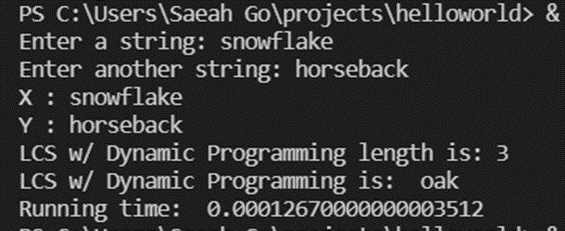
\includegraphics[scale = 0.7]{case1 DP.png} \\
\end{center}
With the dynamic programming implementation, we get $0.0001267$ seconds for the running time.
\subsubsection{Brute Force}
\begin{center}
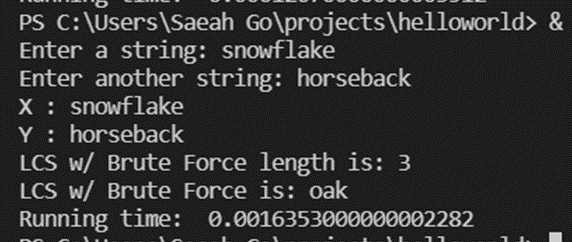
\includegraphics[scale = 0.7]{case1 BF.png} \\
\end{center}
With the brute force implementation, we got $0.00163530$ seconds. We can see that the running time of the brute force version is bigger than the dynamic programming one.

\subsection{\textbf{Case 2}} 
In the second case, we have two strings, ``ABCDGHAKCHFKSJHKJDGH" and ``AEDFHRKOSNCKFJFD", and each string length is 20 and 16. The longest common subsequence is ``ADFKSKJD", and its length is 8.
\subsubsection{Dynamic Programming}
\begin{center}
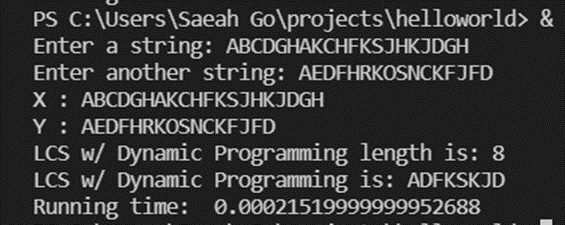
\includegraphics[scale = 0.7]{case2 DP.png} \\
\end{center}
We got about $0.00021519999$ seconds for the implementation with dynamic programming. We can check that we got a bigger running time compare to Case 1 with dynamic programming version.
\subsubsection{Brute Force}
\begin{center}
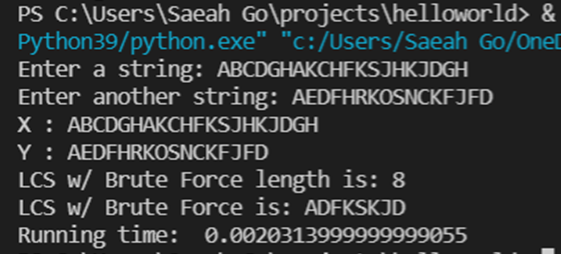
\includegraphics[scale = 0.7]{case2 BF.png} \\
\end{center}
We got $0.002031999$ seconds with the brute force method. We can observe that the time execution is higher than the Case 1 with brute force implementation. ($0.002031999s > 0.00163530s$) Also we can check that the brute force version's execution time is much bigger than the dynamic programming version's. ($0.002031999 > 0.00021519999$)

\subsection{\textbf{Case 3}} 
In this case, the first string, X, is ``springtimemaelstromheroicallysnowflake" (length 38) and the second string Y is ``pioneerbecalmscholarlyhorseback" (length 31). Its LCS is ``pineerecalsolae" (length 15).
\subsubsection{Dynamic Programming}
\begin{center}
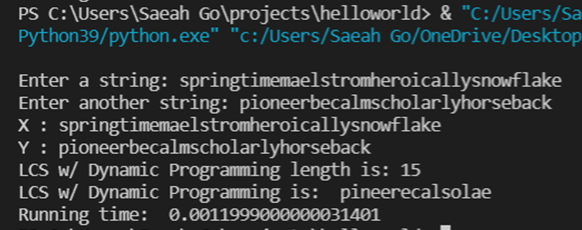
\includegraphics[scale = 0.7]{case3 DP.png} \\
\end{center}
We have $0.00119990000000314$ seconds with the dynamic programming algorithm. We can see that the elapsed time is bigger compare to Case 2's dynamic programming algorithm. 
\subsubsection{Brute Force}
\begin{center}
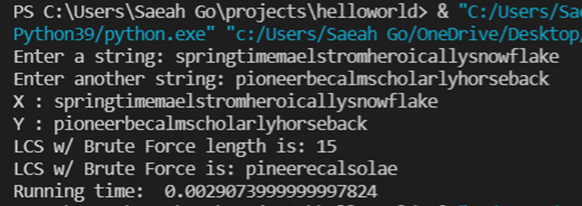
\includegraphics[scale = 0.7]{case3 BF.png} \\
\end{center}
We got $0.00290739999999978s$ for the brute force version, we can also check that the running time in this case is bigger than the DP version and Case 3's brute force version. 

\subsection{\textbf{Case 4}} 
Case 4 has X which length is 43 and the string is ``pkvrrmkikvicuxnugdiuwtwpghcubmfhahkbwbmvwhe". For Y, its length is also 43 and the string is ``cpfbdpmrduymankptxwaxdvvjtqeykwgjedrmvmfuyi". In this case, the LCS is ``cdpumakwvwe" and its length is 11.
\subsubsection{Dynamic Programming}
\begin{center}
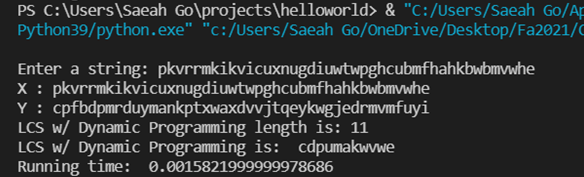
\includegraphics[scale = 0.7]{case4 DP.png} \\
\end{center}
We get $0.00158219999999786$ seconds in this case. We can check that the running time is smaller than the brute force version ($0.00326819999999905$ seconds), but it is bigger than the Case 3 dynammic programming version ($0.00119990000000314$) which makes sense to me since this case's input sizes (string sizes) are bigger compare to Case 3.
\subsubsection{Brute Force}
\begin{center}
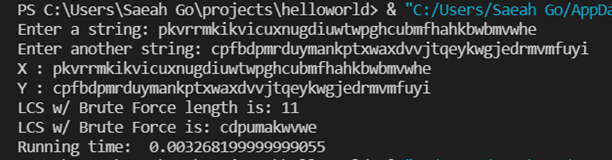
\includegraphics[scale = 0.7]{case4 BF.png} \\
\end{center}
The running time in this case is $0.00326819999999905$. We can see that the elapsed time is bigger than Case 3's brute force version, which is  $0.00290739999999978$. And as mentioned above, time execution of Case 4's brute force version is bigger than Case 4's dynamic programming version.


\subsection{\textbf{Case 5}} 
For the last case, we considered longest strings, which are ``ftzzzikkqgjhtqrgiikigthbbtqjianaraiqbfjdzqvqeqejphfbzwe" and 
``tvcgegziujpxtgrufxwtiqnwtyphtmyqehqgqtgxcbczviycdntnwbjbai". Their length sizes are 55 and 58 each, and the LCS is ``tzijtgithtqqbzvjb" with length 17.
\subsubsection{Dynamic Programming}
\begin{center}
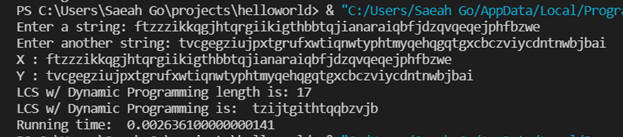
\includegraphics[scale = 0.7]{case5 DP.png} \\
\end{center}
In this case, we got 0.00263610000000014 with the dynamic programming implementation.
\subsubsection{Brute Force}
\begin{center}
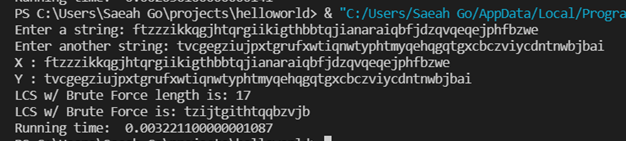
\includegraphics[scale = 0.7]{case5 BF.png} \\
\end{center}
We got 0.00322110000000108 seconds for this brute force implementation case.

\section{\textbf{Analysis Results}}
\indent Based on the test performance results, we made a graph in R and we got: \\
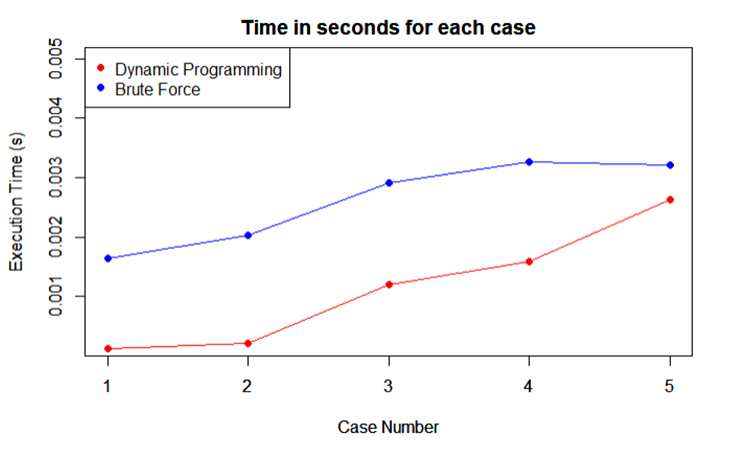
\includegraphics[scale = 0.65]{graph.png} \\
\indent To explain what the case number denotes briefly, Case 1 has the smallest input size, 9 for both strings. As the case number bigger the string input sizes get bigger too. In other words, as the case number increases, the input sizes increase as well. So for the Case 5, we have the longest inputs, 55 and 58. In the graph we could check that the running time of the implementation of dynamic programming method (the red dots and the red line) is strictly smaller than the running time of the implementation of brute force method (the blue dots and the blue line). We can clearly see that using dynamic programming is more efficient than using brute force method. Overall the performance testing went well and we got reasonable values of the running time. We saw the results what we expected before the experiment.

\section{\textbf{Recommendations}}
\indent As we can see in the Analysis Results part, if we implement a problem with brute force algorithm, the running time is higher compare to the solution with dynamic programming algorithm. And we can check this theoretically. With the brute force, its time efficiency is $O(2^n)$, when $n$ is the length of shorter string and with the dynamic programming its time complexity is $O(mn)$, where $m,n$ are the lengths of the two input strings. It makes sense since $O(2^n) \ge O(mn)$, dynamic programming method is more efficient than the brute force method. So I recommend using dynamic programming rather than brute force algorithm.

\section{\textbf{Appendix 1}} 
\begin{center}
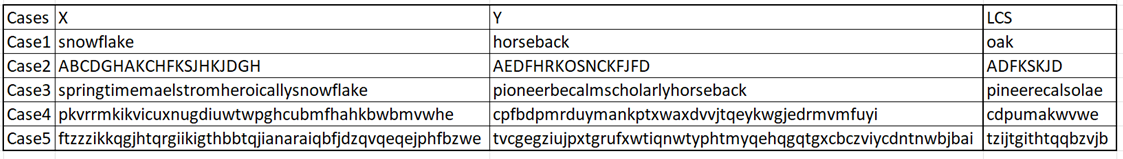
\includegraphics[scale = 0.4]{table1} \\
\scriptsize{Table 1}
\end{center}
\indent This table shows total three strings, the two strings we considered and one output string (LCS) in the performance testing. The first column (The Cases column) indicates the case number in the graph above in the Analysis Results. More precisely, those are the case numbers which is used when creating a graph. The second column, X, indicates the first string input. Similarly, the third column Y indicates the second string input. The last column, LCS, shows the longest common subsequences we got as the output during the experiment. 

\begin{center}
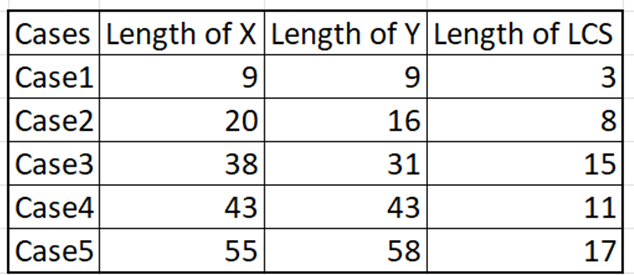
\includegraphics[scale = 0.4]{table2} \\
\scriptsize{Table 2}
\end{center}
\indent We also first included the column Cases, as we did in the first table, to make sure this table considered the same cases with the table above. Each case number indicates the same case. The second column, Length of X shows the length of the first string (X). Similarly, the third column Length of Y shows the length of the second string (Y). Lastly, the fourth column Length of LCS shows the length of the output, LCS.

\begin{center}
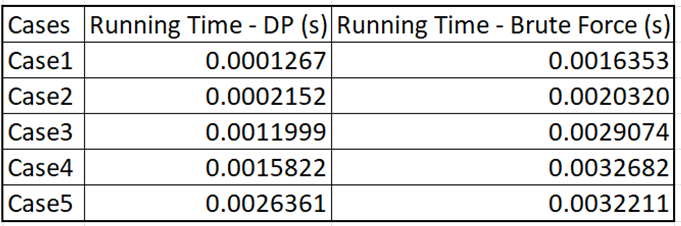
\includegraphics[scale = 0.5]{table3}\\
\scriptsize{Table 3}
\end{center}
This table also includes the Case column. The Running Time - DP (s) column indicates the running time when we implement with dynamic programming. Since we record time execution, the unit is seconds, shortly s. Similarly, the Running Time - Brute Force (s) column shows the execution time of brute force implementation. We can see that the values of the second column (DP) is much smaller than the third column (Brute Force) and as the input strings sizes get bigger the time it took when we are testing also get bigger. 

\section{\textbf{Appendix 2}}
\indent Our first case input is $snowflake$, which input size is 9. Our another input is $horseback$, and its size is also 9. The strings only consists of all lowercase. We wanted to start from the small amounts of input. \\ 
\indent The second case's strings are $ABCDGHAKCHFKSJHKJDGH$ and $AEDFHRKOSNCKFJFD$. Their size are 20 and 16 each, which are a little bigger than the first case. We thought it's a reasonable length to see the time complexity. This time, the two strings only includes uppercase letters. \\
\indent The third case's strings are $springtimemaelstromheroicallysnowflake$ and $pioneerbecalmscholarlyhorseback$. These two strings consist of only lowercases, and these sizes are 38 and 31. \\
\indent For the Case 4 input strings, we choose $pkvrrmkikvicuxnugdiuwtwpghcubmfhahkbwbmvwhe$ and $cpfbdpmrduymankptxwaxdvvjtqeykwgjedrmvmfuyi$. Somewhat no make sense sentence, but we wanted to consider a string which lengths are about 40s. So the length of the string is 43.\\
\indent For the last case's strings, we chose $ftzzzikkqgjhtqrgiikigthbbtqjianaraiqbfjdzqvqeqejphfbzwe$ and $tvcgegziujpxtgrufxwtiqnwtyphtmyqehqgqtgxcbczviycdntnwbjbai$. The strings only consist of lower case letters, and the string lengths are 55 and 58, the most longest strings among our test cases. \\
\indent For more detailed descriptions of inputs and its size, please check the table 1 in Appendix 1.
\end{document}